\chapter{Long-Lived Particles in ATLAS}

\label{ch:simulation}
% --------------------------------------------------------------------------------

As discussed in Section~\ref{sec:limitations}, various limitations in the \ac{SM} suggest a need for new particles at the \TeV scale. 
A wide range of extensions to the \acl{SM} predict that these new particles can have lifetimes greater than approximately one-hundredth of a nanosecond.
These include theories with universal extra-dimensions~\cite{extra_dim1, extra_dim2}, with new fermions~\cite{newfermions}, and with leptoquarks~\cite{leptoquark}.
As discussed in Section~\ref{sec:llp_theory}, many \ac{SUSY} theories also produce these \acp{LLP}, in both R-Parity violating~\cite{rpv1, rpv2, rpv3} and R-Parity conserving~\cite{rpc1, rpc2, rpc3, rpc4} formulations.
Split supersymmetry~\cite{split1, split2}, for example, predicts long-lived gluinos with O(\TeV) masses.
This search focuses specifically on the \ac{SUSY} case, but many of the results are generic to any model with \acp{LLP}. 

Long-lived gluinos or squarks carry color-charge and will thus hadronize into color neutral bound states called \rhadrons.
These are composit particles like the known hadrons but with one supersymmetric constituent, for example $\tilde{g}q\bar{q}$ and $\tilde{q}\bar{q}$.
In this hadronization process, the gluino can acquire an electric charge.
Gluino pair production, $p p\rightarrow \tilde{g}\tilde{g} + X$, where X denotes the proton remnants, has the largest cross sectional increase with the increase in energy to 13 TeV, and so this search uses gluino \rhadrons as its benchmark model.
The features, techniques, and cross section limits discussed here are all largely independent of the model.
Planned future updates will extend the case to include additional refinements for squark and chargino models, but the current method covers any long-lived, charged, massive particle.

\section{Event Topology}
\label{sec:characteristics}

R-parity conserving  SUSY models predict that gluinos will be produced in pairs at the \ac{LHC}, through the processes shown in Figure~\ref{fig:gluino_pair}, where the quarks and gluons are proton constituents.
The gluon-initiated mode dominates for the collision energy and gluino masses considered for this search.
During their production, the long-lived gluinos hadronize into color singlet bound states including $\tilde{g}q\bar{q}$ and even $\tilde{g}g$~\cite{rhadron}.
The probability to form the gluon-only bound states is a free parameter usually taken to be 0.1, and 90\% of the remaining \rhadrons form meson states~\cite{rhad_atlas}.
The charged and neutral states are approximately equally likely for mesons, so the \rhadrons will be charged roughly 50\% of the time.

\begin{figure}
\centering
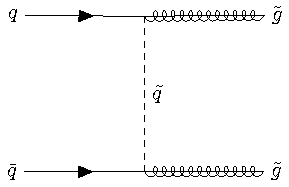
\includegraphics[width=\halffig]{figures/qq_t_gluinos.pdf}
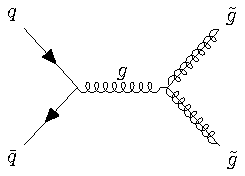
\includegraphics[width=\halffig]{figures/qq_s_gluinos.pdf}\\
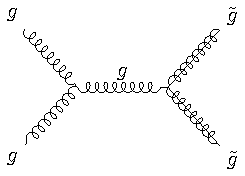
\includegraphics[width=\halffig]{figures/gg_gluinos.pdf}
\caption{The processes which contribute to gluino pair production in the proton proton collisions, where the quarks and gluons are proton constituents.}
\label{fig:gluino_pair}
\end{figure}

These channels produce \rhadrons with large \pt, but lower on average than their mass, so that they typically propagate with $0.2 < \beta < 0.9$~\cite{rhad_atlas}.
Figure~\ref{fig:rhad_truth} shows the generated \pt and $\beta$ distributions for a simulated example of \rhadrons with a mass of 1600 \GeV.
The mean \pt is roughly half of the mass at 800 \GeV, and so $\beta$ peaks around 0.5.
The fragmentation that produces that hadrons is very hard, so the jet structure around the \rhadron is minimal, with less than 5 \GeV of summed particle momentum expected in a cone of $\Delta R < 0.25$ around the \rhadron~\cite{rhad_atlas}.
After hadronization, depending on the gluino lifetime, the \rhadrons then decay into hadrons and a \ac{LSP}~\cite{rhadron}.

\begin{figure}
\centering
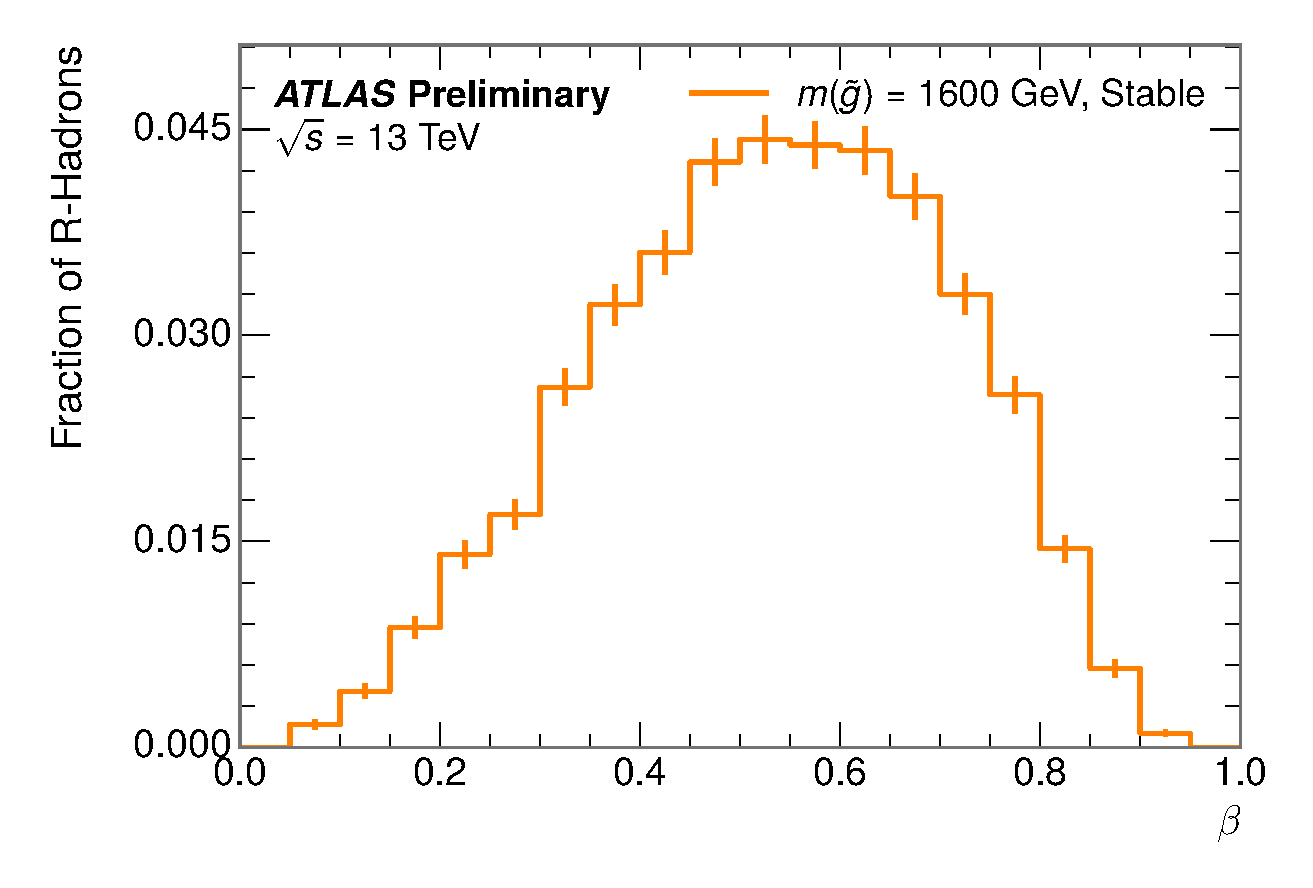
\includegraphics[width=\halffig]{figures/rhad_beta.pdf}
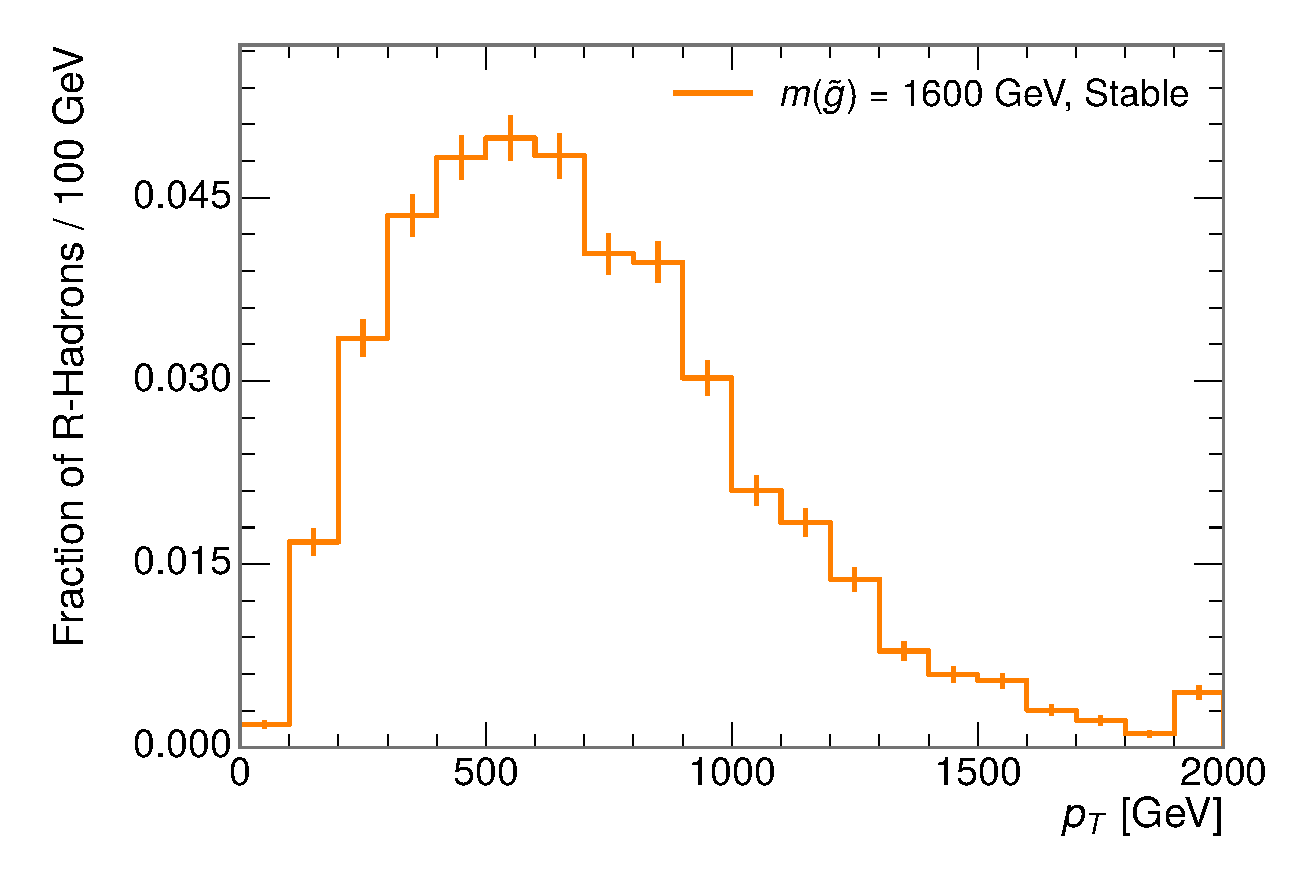
\includegraphics[width=\halffig]{figures/rhad_pt.pdf}
\caption{The generated \pt and $\beta$ distributions for \rhadrons with $M = 1600\ \GeV$.}
\label{fig:rhad_truth}
\end{figure}

In summary, the expected event for pair-produced long-lived gluinos is very simple: two isolated, high-momentum \rhadrons that propagate through the detector before decaying to jets.
The observable features of such events depend strongly on the interaction of the \rhadron with the material of the detector and also its lifetime.
Section~\ref{sec:rh_interactions} describes the interactions of \rhadrons which reach the various detector elements in ATLAS and Section~\ref{sec:rh_lifetimes} provides a summary of the observable event descriptions for \rhadrons of various lifetimes.

\subsection{Detector Interactions}
\label{sec:rh_interactions}

Although the distribution of decay times can be parametrized with a single parameter, $\tau$, the time before individual \rhadrons decay follows an exponential distribution, leading to a range of decay times for any individual lifetime.
This is further confounded by the distribution of $\beta$ as well as $\eta$, so that each \rhadron propagates at a different velocity and travels a different distance before reaching each detector element.
Therefore, the lifetime-dependent event topologies must be discussed as an average, and all times referred to within this section will assume $\beta = 0.5$, an $\eta = 0$, and that the particle decays after a time equal to its lifetime.
Table~\ref{tab:detector_times} lists the distances of various subdetectors and the time after which a \ac{LLP} will arrive at that subdetector for a few values of $\beta$ and with $\eta = 0$.

\begin{table}[h!]
\begin{tabular}{lcccc}
\hline
Subdetector & Distance & $\tau$ at $\beta = 0.3$ & $\tau$ at $\beta = 0.5$ & $\tau$ at $\beta = 0.7$ \\
\hline
Pixel & 3.1 cm & 0.35 ns & 0.20 ns & 0.15 ns\\
Calorimeter & 1.5 m & 17 ns & 10 ns & 7.2 ns \\
Muon System & 5 m & 56 ns & 33 ns & 24 ns \\
\hline
\end{tabular}
\caption{The radial distances of each of the subdetectors and example arrival times for an \rhadron with $\eta = 0$ and the specified $\beta$.}
\label{tab:detector_times}
\end{table}

After approximately 0.2 ns, the \rhadron reaches the first layer of the pixel detector. If charged, it deposits energy into the material through repeated single collisions that result in ionization of the silicon substrate~\cite{pdg}. 
Because of its comparatively low $\beta$, the ionization energy can be significantly greater than expected for \ac{SM} particles because the most-probable energy loss grows significantly as $\beta$ decreases~\cite{pdg}.
This large ionization can be measured through the \ac{ToT} read out from the pixel detector as described in Section~\ref{sec:pixel_dedx}.
Large ionization in the inner detector is one of the major characteristic features of \acp{LLP}.
The particle propagates through all four layers of the pixel detector, where each provides a measurement of ionization, and then exits the pixel detector at 0.8 ns.

Throughout the next few nanoseconds, the \rhadron propagates through the remainder of the inner detector.
A charged \rhadron will provide hits in each of these systems as would any other charged particle, and can be reconstructed as a track.
The track reconstruction provides a measurement of its trajectory and thus its $p$ as described in Section~\ref{sec:tracks}.
The large $p_T$, shown in Figure~\ref{fig:rhad_truth}, is another characteristic feature of massive particles produced at the \ac{LHC}.

As of roughly 10 ns, the \rhadron enters the calorimeter where it interacts hadronically with the material.
Because of its large mass and $p$, the \rhadron does not typically stop in the calorimeter, but rather deposits a small fraction of its energy through repeated interactions with nucleons.
The probability of interaction between the gluino itself and a nucleon is low because the cross section drops off with the inverse square of its mass, so the interactions are primarily governed by the light constituents~\cite{g4_rhad_2009}.
Each of these interactions can potentially change that quark content and thus change the sign of the \rhadron, so that the charge at exit is typically uncorrelated with the charge at entry~\cite{rhad_atlas}.
The total energy deposited in the calorimeters during the propagation is small compared to the kinetic energy of the \rhadron, around 20-40 \GeV, so that \ep is typically less than 0.1~\cite{rhad_atlas}.

Then, 30 ns after the collision, it reaches the muon system, where it again ionizes in the material if charged and can be reconstructed as a muon track.
Because of the charge-flipping interactions in the calorimeter, this track may have the opposite sign of the track reconstructed in the inner detector, or there may be a track present when there was none in the inner detector and vice-versa for those which are detected.
The propagation time at the typically lower $\beta$ results in a significant delay compared to muons, and a delay over 25 ns causes the muon signal to be lost outside the readout window.
Between the probability of charge-flip and late arrival, there is a significant chance that an \rhadron which was produced with a charge will not be identified as a muon.
When it is reconstructed as a muon, that delay can be assessed in terms of a time-of-flight measurement, which is another characteristic feature of \rhadrons.

\subsection{Lifetime Dependence}
\label{sec:rh_lifetimes}

The above description assumed a lifetime long enough for the \rhadron to exit the detector, which through this search is referred to as \ac{VLL}, as the particle may decay after exiting the detector.
There are several unique signatures at shorter lifetimes where the \rhadron decays in various parts of the inner detector; these lifetimes are referred to as \ac{LL}.

The shortest case where the \rhadron is considered \ac{LL} is for lifetimes around 0.01 ns, where the particle decays before reaching any of the detector elements.
Although the \rhadrons are produced opposite each other in the transverse plane, each \rhadron decays to a jet and an \ac{LSP}.
The two decays are uncorrelated, so the two \acp{LSP} carry different momenta and in different directions. 
And, since the \acp{LSP} are not measured, the produced jets can be significantly imbalanced in the transverse plane which results in large missing energy.
That missing energy can be used to trigger candidate events, and provides the most efficient trigger option for shorter lifetimes.
Additionally, the precision of the tracking system allows the displaced vertex of the \rhadron decay to be reconstructed from the charged particles in the jet.
The distance of that vertex from the interaction point can be used to distinguish \rhadron decays from other processes.
Figure~\ref{fig:rhadron_displaced} shows a schematic diagram of an example \rhadron event with such a lifetime.
The diagram is not to scale, but instead illustrates the detector interactions in the pixel detector, calorimeters, and muon system.
It includes a representation of a charged \rhadron and a neutral \rhadron, as well as the \acp{LSP} and jets (shown as charged hadrons) produced in the decay.
Neutral hadrons may also be produced in the decay but are not depicted.
Previous searches on ATLAS have used the displaced vertex to target \ac{LLP} decays~\cite{SUSY-2014-02}.

\begin{figure}[tb]
\centering
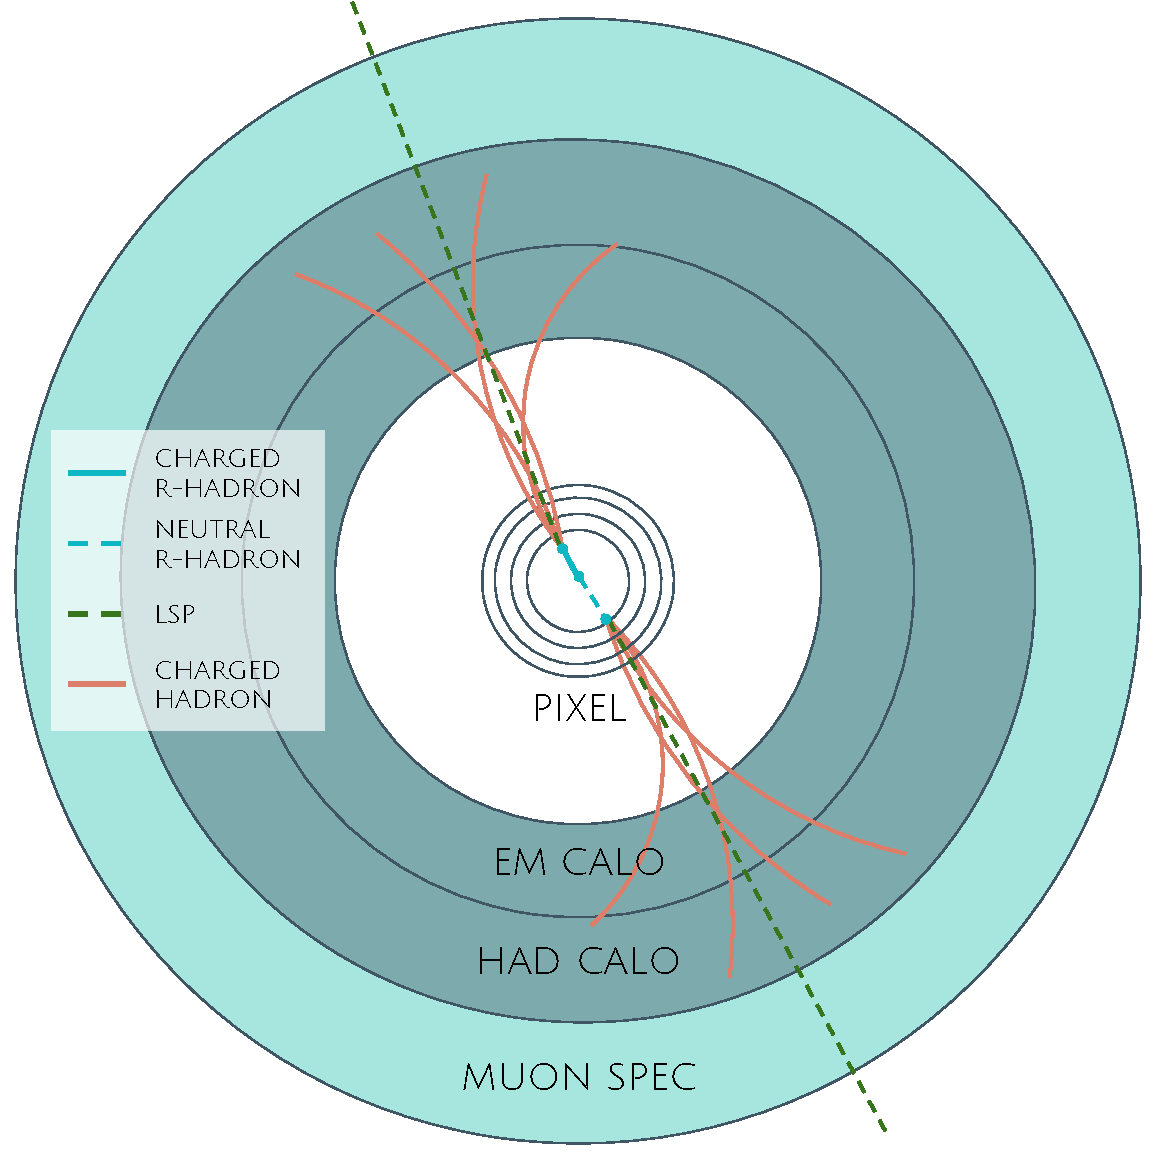
\includegraphics[width=\fullfig]{figures/rhadron_displaced.pdf}
\caption{A schematic diagram of an \rhadron event with a lifetime around 0.01 ns. The diagram includes one charged \rhadron (solid blue), one neutral \rhadron (dashed blue), \acsp*{LSP} (dashed green) and charged hadrons (solid orange). The pixel detector, calorimeters, and muon system are illustrated but not to scale.}
\label{fig:rhadron_displaced}
\end{figure}

The next distinguishable case occurs at lifetimes greater than 0.1 ns but less than 10 ns, where the \rhadron forms a partial track in the inner detector.
This forms a unique signature of a disappearing track.
Two examples of such an event are illustrated in Figure~\ref{fig:rhadron_disappear} and Figure~\ref{fig:rhadron_metastable_short}, which show the short track in the inner detector.
The decay distance must be sufficiently long that it reaches the \ac{SCT}, or else to track will not be reconstructed at all.
Depending on the mass difference between the \rhadron and the \ac{LSP}, the decay products will either be a single, soft charged hadron and a \ac{LSP} (Figure~\ref{fig:rhadron_disappear}), or a jet and a \ac{LSP} (Figure~\ref{fig:rhadron_metastable_short}).
A dedicated search on ATLAS used the disappearing track signature  in the former case to search for \ac{LLP} in Run 1~\cite{SUSY-2013-01}.

In the latter case, the decays result in an event-level signature of up to two high-$p$ tracks, jets, and significant missing energy.
The missing energy has the same origin as in the case of 0.01 ns lifetimes, from the decay to unmeasured particles, and again can be large.
The high-$p$ tracks will also have the characteristicly high-ioniziation of massive, long-lived paticles in the Pixel detector.
Figure~\ref{fig:rhadron_metastable_short} shows how the jets from the decay can still be reconstructed in the calorimeter.
Several previous searches on ATLAS from Run 1 have used this signature to search for \rhadrons~\cite{SUSY-2012-01, SUSY-2013-22}, including a dedicated search for \ac{LL} particles~\cite{SUSY-2014-09}.

\begin{figure}[tb]
\centering
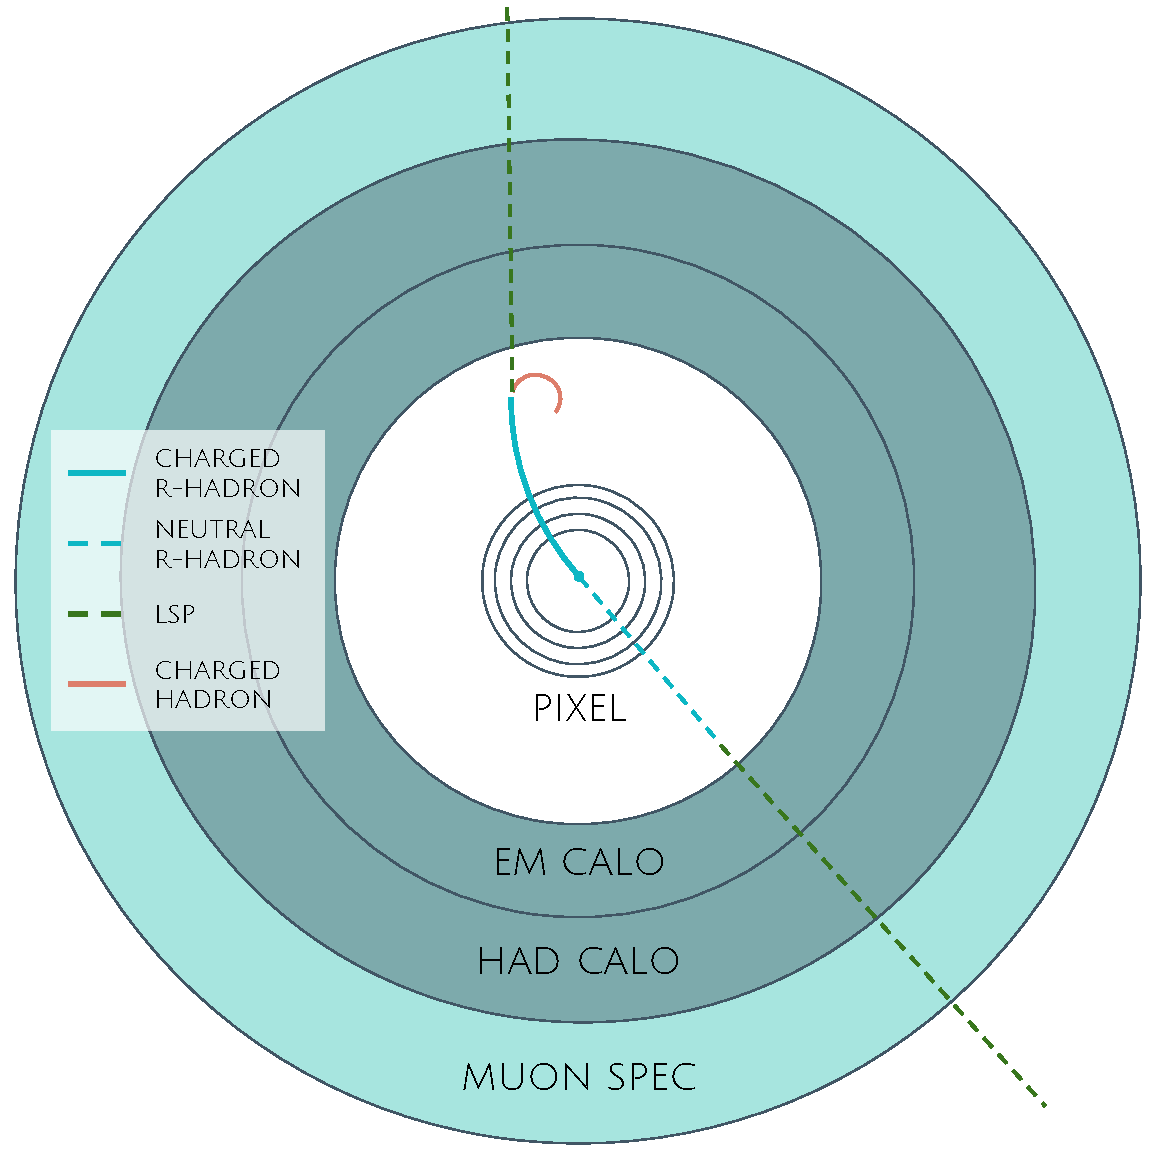
\includegraphics[width=\fullfig]{figures/rhadron_disappear.pdf}
\caption{Schematic diagram of an \rhadron event with a lifetime around 5 ns, where the masses of the \rhadron and \acs*{LSP} are nearly degenerate. The diagram includes charged \rhadrons (solid blue), neutral \rhadrons (dashed blue), \acsp*{LSP} (dashed green) and charged hadrons (solid orange). The pixel detector, calorimeters, and muon system are illustrated but not to scale.}
\label{fig:rhadron_disappear}
\end{figure}

\begin{figure}[tb]
\centering
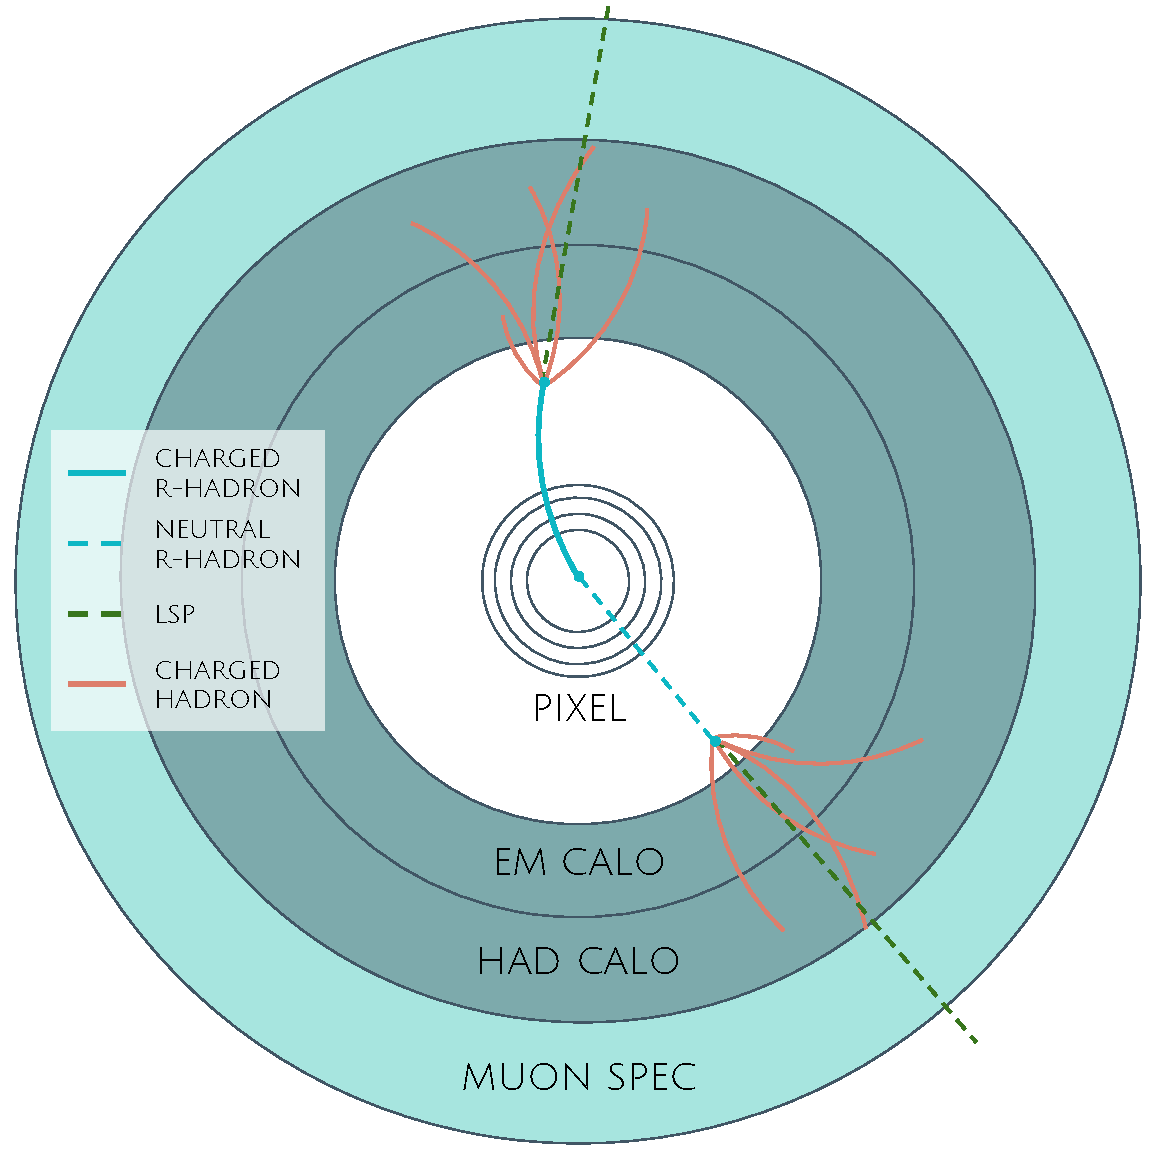
\includegraphics[width=\fullfig]{figures/rhadron_metastable_short.pdf}
\caption{Schematic diagram of an \rhadron event with a lifetime around 5 ns, where the masses of the \rhadron and \acs*{LSP} are not degenerate. The diagram includes charged \rhadrons (solid blue), neutral \rhadrons (dashed blue), \acsp*{LSP} (dashed green) and charged hadrons (solid orange). The pixel detector, calorimeters, and muon system are illustrated but not to scale.}
\label{fig:rhadron_metastable_short}
\end{figure}

If the lifetime is longer than several nanoseconds, in the range of 10-30 ns, the \rhadron decay can occur in or after the calorimeters, but prior to reaching the muon system.
In the case that the decays occur early enough within the calorimeters that the decay can be measured, the event topology is very similar to the above with jets originating in the inner detector.
If the decay occurs after the calorimeter, jets may not be reconstructed at all.
The events still often have large missing energy, although it is generated through different mechanisms, and so the same search strategy can be used.
The \rhadrons do not deposit much energy in the calorimeters, so a neutral \rhadron will not enter into the missing energy calculation.
A charged \rhadron opposite a neutral \rhadron will thus generate significant missing energy, and close to 50\% of pair-produced \rhadron events fall into this category.
If both \rhadrons are neutral then the missing energy will be low because neither is detected.
Two charged \rhadrons will also result in low missing energy because both are reconstructed as tracks and will balance each other in the transverse plane.
A small fraction of the time, one of the charged \rhadron tracks may fail quality requirements and thus be excluded from the missing energy calculation and again result in signficant missing energy.
Figure~\ref{fig:rhadron_metastable_long} illustrates another example event with one charged \rhadron which decays after approximately 20 ns, and shows how the jets from the decay might not be reconstructed.

\begin{figure}[tb]
\centering
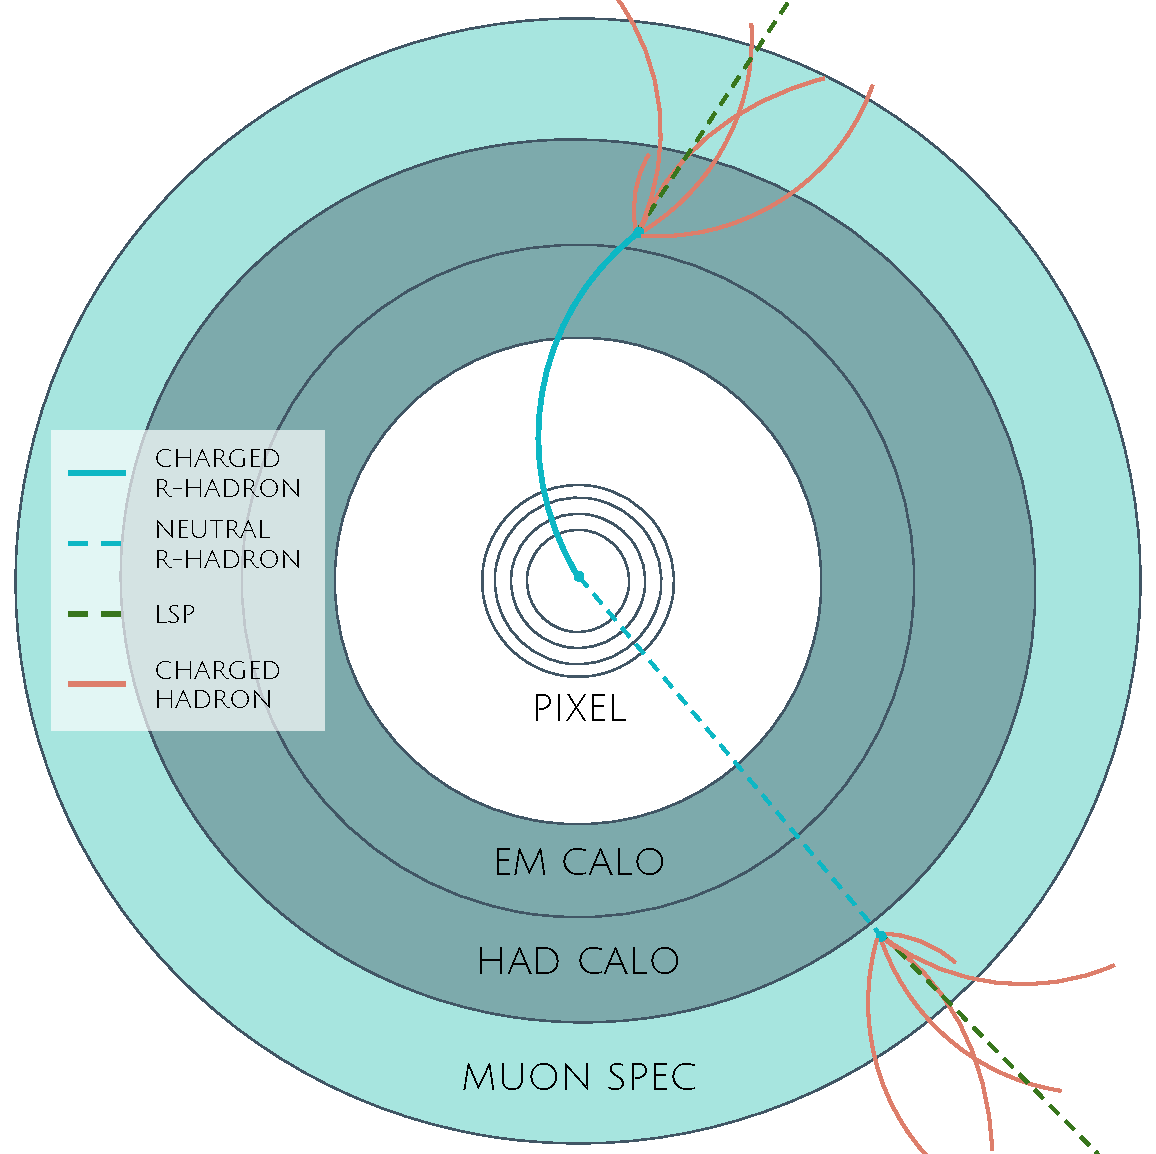
\includegraphics[width=\fullfig]{figures/rhadron_metastable_long.pdf}
\caption{A schematic diagram of an \rhadron event with a lifetime around 20 ns. The diagram includes one charged \rhadron (solid blue), one neutral \rhadron (dashed blue), \acsp*{LSP} (dashed green) and charged hadrons (solid orange). The pixel detector, calorimeters, and muon system are illustrated but not to scale.}
\label{fig:rhadron_metastable_long}
\end{figure}


The longest lifetimes, the \ac{VLL} case, has all of the features of the 30-50 ns case but with the addition of muon tracks for any \rhadrons that exit the calorimeter with a charge.
That muon track can provide additional information from time-of-flight measurements to help identify \acp{LLP}.
An example of the event topology for one charged and one neutral \ac{VLL} \rhadron is shown in Figure~\ref{fig:rhadron_stable}.
Some searches on ATLAS have included this information to improve the search reach for \ac{VLL} particles~\cite{SUSY-2013-22, stable2016}.

\begin{figure}[tb]
\centering
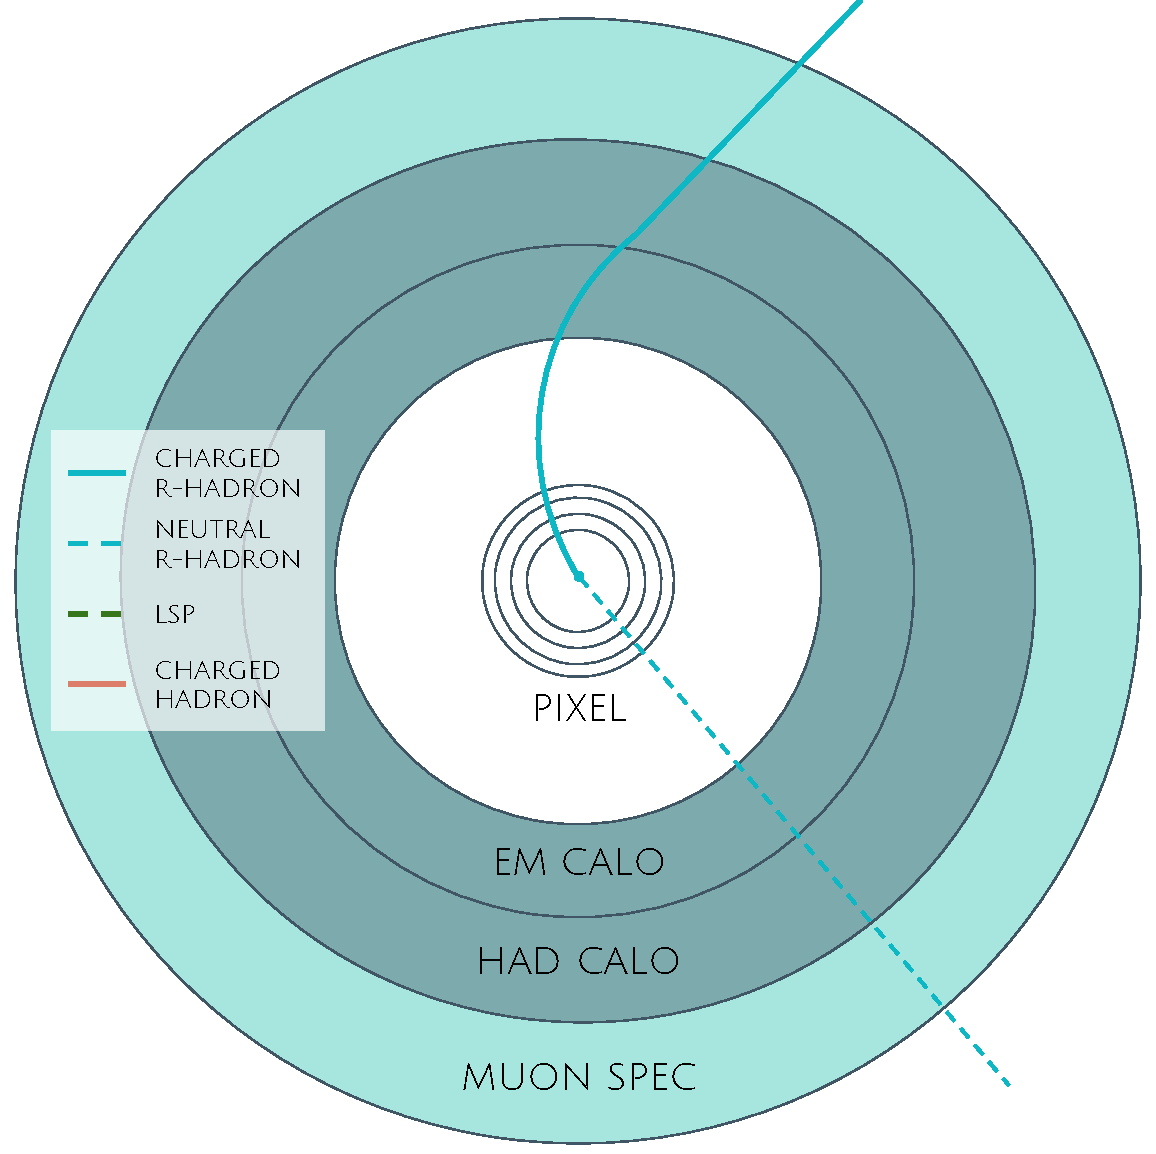
\includegraphics[width=\fullfig]{figures/rhadron_stable.pdf}
\caption{A schematic diagram of a \acs*{VLL} \rhadron event. The diagram includes one charged \rhadron (solid blue) and one neutral \rhadron (dashed blue). The pixel detector, calorimeters, and muon system are illustrated but not to scale.}
\label{fig:rhadron_stable}
\end{figure}


% ----------------------------------------

\section{Simulation}
\label{sec:simulation_samples}

All of the event topologies discussed above are modeled by simulations of \rhadron events in the ATLAS detector. 
A large number of such samples are generated to determine efficiencies, to measure expected yields, and to estimate uncertainties. 
The primary interaction, pair production of gluinos with masses between 400 and 3000 \GeV, is simulated using \texttt{Pythia 6.4.27}~\cite{pythia6}  with the AUET2B~\cite{ATL-PHYS-PUB-2011-014} set of tuned parameters for the underlying event and the CTEQ6L1 \cite{CTEQ} \ac{PDF} set.
The simulated interactions include a modeling of pileup by adding secondary, minimum bias interactions from both the same (in-time pileup) and nearby (out-of-time pileup) bunch crossings.
This event generation is then augmented with a dedicated hadronization routine to hadronize the long-lived gluinos into final states with \rhadrons~\cite{heavy_hadronization}, with the probability to form a gluon-gluino bound set at 10\%~\cite{Fairbairn:2006gg}.

The cross sections used for these processes are calculated at \ac{NLO} in the strong coupling constant with a resummation of soft-gluon emmision at \ac{NLL}~\cite{Beenakker:1996ch,Kulesza:2008jb,Kulesza:2009kq,Beenakker:2009ha,Beenakker:2011fu}.
The nominal predictions and the uncertainties for each mass point are taken from an envelope of cross-section predictions using different \ac{PDF} sets and factorization and renormalization scales~\cite{Kramer:2012bx}.
As discussed in Section~\ref{sec:ppcollisions}, the \acp{PDF} and scales determine the cross section by providing the probabilities of the proton constituents to interact.
Multiple estimates for the \ac{PDF} and scales at 13 \TeV can be used to provide an average cross section calculation and its uncertainty.

The \rhadrons then undergo a full detector simulation~\cite{SOFT-2010-01}, where the interactions of the \rhadrons with the material of the detector are described by dedicated \texttt{Geant4}~\cite{GEANT4} routines. 
These routines model the interactions described in Section~\ref{sec:rh_interactions}, including the ionizing interactions in the silicon modules of the inner detector and the \rhadron-nucleon interactions in the calorimeters~\cite{Mackeprang:2006gx, Mackeprang:2009ad}.
The specific routine chosen to describe the interactions of the \rhadrons with nucleons, the ``generic model'', uses a pragmatic approach where the scattering cross section is taken to be a constant 12 mb per light quark.
In this model the gluino itself does not interact at all, although it carries most of the kinetic energy of the bound state.

The lifetimes of these \rhadrons are then simulated at several working points, $\tau = 0.1, 1.0, 3.0, 10, 30, 50$ and $> 50 ns$.
The actual decay times follow an exponential distribution, where $\tau$ is the characteristic time.
Only one decay mode is simulated for these benchmark samples, $\tilde{g} \rightarrow q\bar{q}\tilde{\chi}_1^0$ with the neutralino mass set to 100 \GeV.
The search discussed here is also efficient for heavier neutralinos, which have very similar topologies but which generate less missing energy.

All of the simulated events are then reconstructed using the same software used for collision data.
The fully reconstructed events are then reweighted to match the distribution of initial state radiation in an alternative sample of events, generated with \texttt{MG5\_aMC@NLO}~\cite{madgraph}, which has had a more accurate description of radiate effects than \texttt{Pythia6} in previous iterations~\cite{SUSY-2014-09}.
\texttt{MG5\_aMC@NLO} predicts a harder distribution of initial state radiation, where 28\% more simulated events generate sufficient missing energy to trigger for \ac{VLL} \rhadrons.
This reweighting provides a more accurate description of the $p$ of the gluino-gluino system and is important in modeling the efficiency of triggering and offline event selection.


% ----------------------------------------
